\chapter{設計}
\label{chap:design}

本章では,本研究におけるコンピュータの構成と,それぞれのコンピュータでどのプログラムを実行するかに関して述べる.

\section{コンピュータの構成}

本研究で実装を行う環境は,RDMA NICが刺さった監視対象ホストと,本研究における実装を実行するホストの2台で構成する.

監視対象ホストは,Linux 4.15.0-72-genericのubuntuであり,PCIeデバイスとして,FPGAボードが刺さっている.
このFPGAボードは,\ref{chap:related_works}章にて述べたように,dma messageとethernetパケットを相互変換する機能を有しており,
インターフェースとして,dma_read関数とdma_write関数がlibtlpに用意されている.
また,このFPGAボードには,IPアドレスとして,192.168.10.1を静的に振ってある.

実装を実行するホストは,Linux 4.19.0-6-amd64のDebian busterであり,光ファイバーケーブル(名称はあとで修正)が刺さるNICを刺している.
このNICにはIPアドレスとして,192.168.10.3を静的に振ってある.
監視対象ホストに対してRDMAを実行する際は,dma_read関数,あるいはdma_wirte関数を通して192.168.10.1に対してIPパケットを送信している.

図\ref{fig:zentai}にて,全体図を書く

\section{物理アドレスを指定したメモリの値の取得}

ここにどのように叩くと値が返ってくるかを書く

\begin{figure}[htbp]
    \caption{全体}
    \label{fig:zentai}
    \begin{center}
        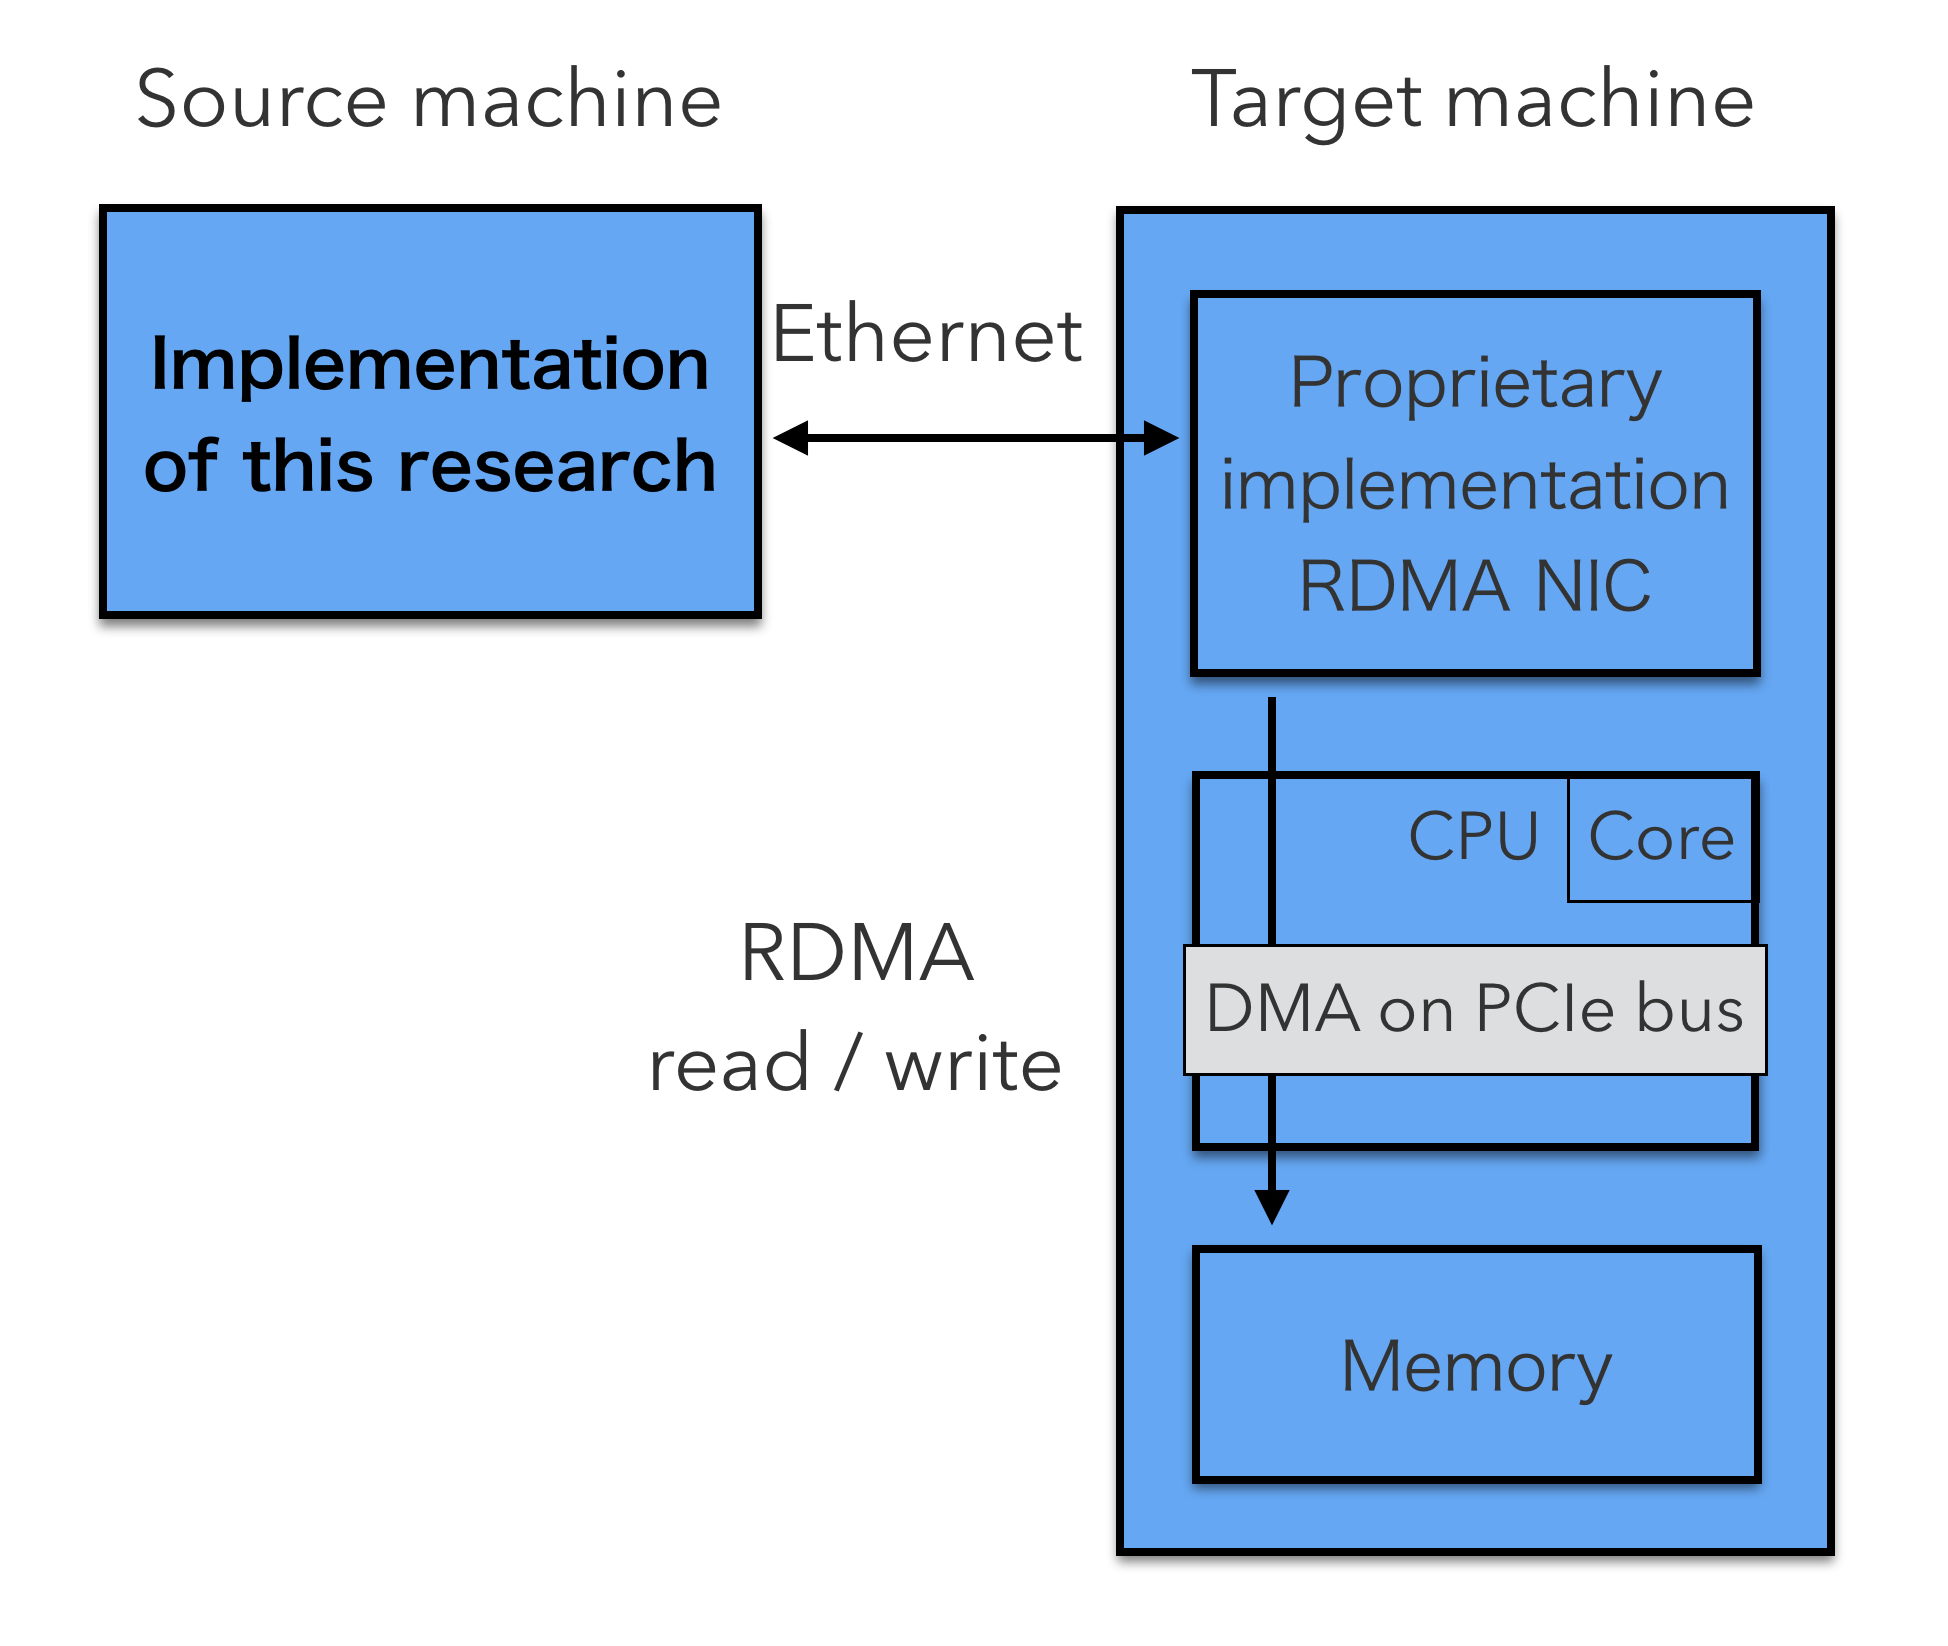
\includegraphics[bb=0 0 1000 530,width=15cm]{img/zentai.png}
    \end{center}
\end{figure}
